\section{Resultados}\label{sec:resultados}

Ambos métodos se corrieron en las 40 semanas BIG con los parámetros de la Sección~\ref{sec:implementacion}. La matheurística tardó en promedio 25 minutos por semana (máximo 44) usando dos hilos, y el caso base menos de un minuto. Todas las soluciones de ambos métodos pasaron la validación independiente: ninguna viola capacidad, compatibilidad, incompatibilidad térmica, ventanas, tiempo máximo de traslado, jornada, capacidad de bases ni capacidad de hubs.

\parrafo{Efecto de las correcciones.} La Tabla~\ref{tab:evolucion} compara las versiones del Informe~2 anterior con las actuales. El caso base corregido cuesta \$3,7 millones menos por semana que el anterior y externaliza 10 solicitudes en vez de 33,6. Eso hace la comparación más exigente: contra el caso base nuevo, la matheurística entregada antes habría ahorrado solo un 1,9\,\%. La matheurística corregida cuesta \$3,1 millones menos por semana que la anterior, con 8 vehículos menos y 4.100 kilómetros menos. Externaliza más que la versión anterior (7,2 contra 3,6 solicitudes), porque ya no contrata vehículos que solo se justifican para atender pocas solicitudes.

\begin{table}[htbp]
\centering
\caption{Promedio semanal en las 40 semanas BIG, antes y después de las correcciones.}\label{tab:evolucion}
\small
\begin{tabular}{lcccc}
\toprule
 & \multicolumn{2}{c}{Caso base} & \multicolumn{2}{c}{Matheurística} \\
\cmidrule(lr){2-3}\cmidrule(lr){4-5}
 & Anterior & Corregido & Anterior & Corregida \\
\midrule
Costo total (MM CLP) & 42,73 & 39,03 & 38,29 & 35,14 \\
Solicitudes externalizadas & 33,6 & 10,0 & 3,6 & 7,2 \\
Vehículos activados & 34,8 & 36,1 & 44,6 & 36,6 \\
Kilómetros & 31.960 & 32.841 & 31.598 & 27.455 \\
Alertas de la validación & -- & 0 & 31 & 6 \\
\bottomrule
\end{tabular}
\end{table}

\parrafo{Comparación global.} La matheurística es más barata que el caso base en las 40 semanas (Figura~\ref{fig:costosemanal}). El ahorro promedio es de 9,9\,\%, con un mínimo de 8,0\,\% y un máximo de 12,9\,\%, lo que equivale a \$3,9 millones por semana o unos \$200 millones al año si la demanda mantiene este patrón. El ahorro no depende de una semana en particular: va de 8,8 a 12,0\,\% entre instancias (Tabla~\ref{tab:instancias}) y no se correlaciona con cuánto externaliza el caso base ($r=-0{,}01$). Es decir, no viene de corregir semanas en que el caso base falla, sino de rutear mejor en todas.

\begin{figure}[htbp]
\centering
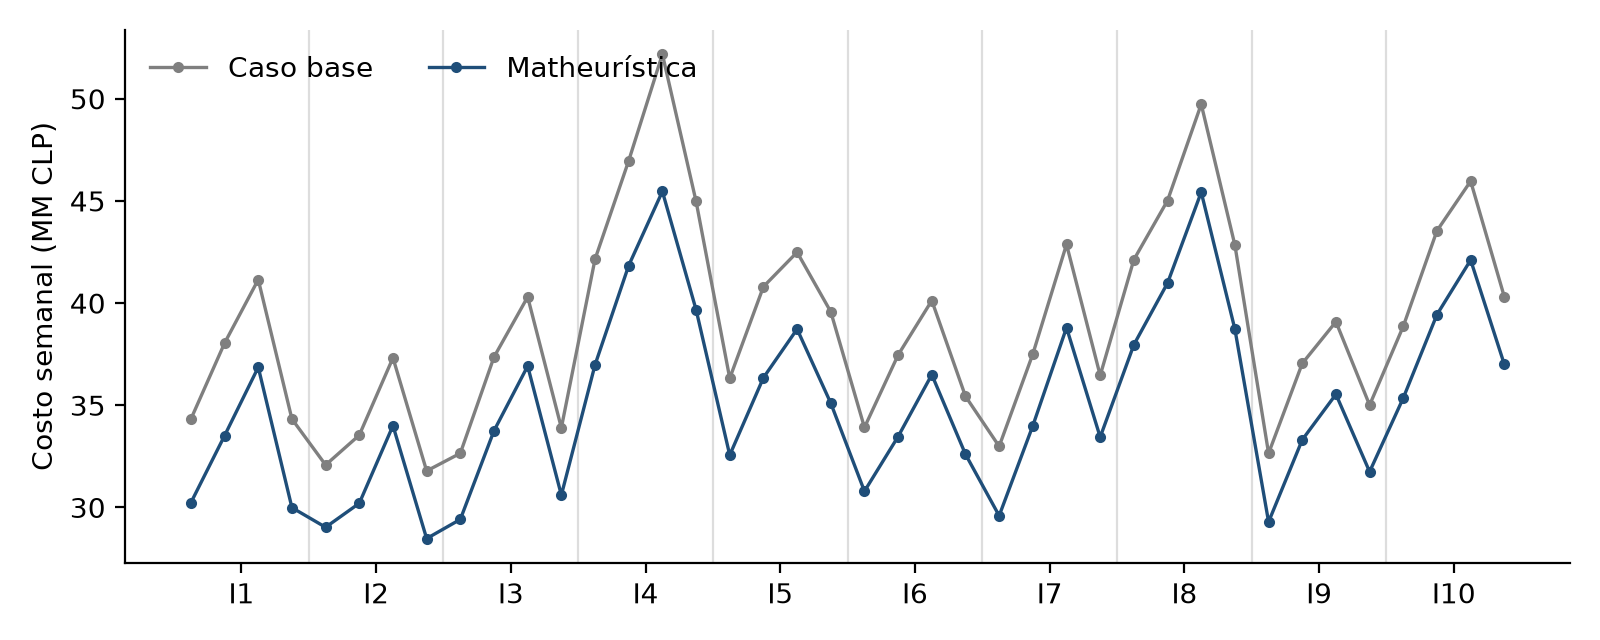
\includegraphics[width=\textwidth]{figures/fig_costo_semanal.png}
\caption{Costo semanal de ambos métodos en las 40 semanas BIG (cuatro semanas por instancia).}\label{fig:costosemanal}
\end{figure}

\begin{table}[htbp]
\centering
\caption{Resultados por instancia (promedio de sus cuatro semanas). Vehículos y externalizadas: caso base / matheurística.}\label{tab:instancias}
\small
\begin{tabular}{ccccccc}
\toprule
Instancia & Solicitudes & \multicolumn{2}{c}{Costo (MM CLP)} & Ahorro & Vehículos & Externalizadas \\
\cmidrule(lr){3-4}
 & por semana & Base & Matheur. & & & \\
\midrule
\tabinput{tablas/instancias.tex}
\bottomrule
\end{tabular}
\end{table}

\parrafo{De dónde viene el ahorro.} La Tabla~\ref{tab:desglose} desglosa el costo. Los kilómetros explican el 84\,\% del ahorro (\$3,26 de \$3,88 millones) y la externalización el 15\,\%; el costo fijo de vehículos sube levemente. La Tabla~\ref{tab:kpisres} muestra el mecanismo. Con casi la misma flota, la matheurística recorre un 16\,\% menos: el factor de recorrido baja de 2,10 a 1,74, es decir, por cada kilómetro que separa el origen y el destino de una solicitud se recorren 1,74 kilómetros en vez de 2,10. Las rutas consolidan más (4,25 tramos por ruta contra 3,99), los vehículos viajan más llenos (40\,\% de uso medio de capacidad contra 36,6\,\%) y recorren menos kilómetros vacíos. El caso base solo agrega cada solicitud a una ruta ya armada sin reordenarla, mientras que el VND y el maestro reordenan y recombinan rutas completas.

\begin{table}[htbp]
\centering
\caption{Desglose del costo semanal promedio (MM CLP).}\label{tab:desglose}
\small
\begin{tabular}{lccccc}
\toprule
Componente & Caso base & \% & Matheurística & \% & Diferencia \\
\midrule
\tabinput{tablas/desglose.tex}
\bottomrule
\end{tabular}
\end{table}

\begin{table}[htbp]
\centering
\caption{Indicadores de desempeño, promedio de las 40 semanas BIG. Los indicadores en porcentaje se comparan en puntos porcentuales (pp).}\label{tab:kpisres}
\small
\begin{tabular}{lccc}
\toprule
Indicador & Caso base & Matheurística & Cambio \\
\midrule
\tabinput{tablas/kpis.tex}
\bottomrule
\end{tabular}
\end{table}

\parrafo{Lo que empeora.} Las entregas atrasadas suben de 0,23 a 0,71\,\% (de 1,3 a 4,1 entregas por semana). Solo se atrasan insumos y equipos, que lo admiten, y el costo total de atraso es el mismo en ambos métodos (\$0,04 millones), porque la penalización por minuto (\$800 y \$1.200) es baja frente al costo de un desvío. Si la organización valora más la puntualidad que lo que indican esas penalizaciones, puede prohibir el atraso: la Sección~\ref{sec:sensres} muestra que hacerlo deja las entregas atrasadas en cero sin subir el costo. Además, el 7,9\,\% de los vehículo-días pagados quedan sin salir (contra 0,4\,\% en el caso base): la matheurística contrata vehículos que se necesitan en los días de mayor demanda y que quedan ociosos el resto de la semana, porque el costo fijo es semanal.

\parrafo{Flota y bases.} Ambos métodos contratan cerca de 8 vans generales, 11,5 vans frías y 17,3 furgones fríos por semana, de 24, 18 y 18 disponibles. El furgón es el recurso escaso: en 26 de las 40 semanas ambos métodos usan los 18, y en esas semanas la matheurística externaliza en promedio 8,3 solicitudes, contra 5,0 en las demás. Es el único vehículo que lleva insumos de más de 30 unidades sin dividirlos, equipos de más de 30 unidades y las cuatro clases a la vez. Ambos métodos usan las 9 bases casi todas las semanas, y la matheurística reparte los vehículos de forma parecida al caso base: mueve medio vehículo hacia Cerrillos y Pudahuel, en el poniente, y lo saca de Quilicura y Macul (Figura~\ref{fig:bases}). Aunque en total se usan unos 37 de los 62 cupos, algunas bases se llenan: Macul y Talagante quedan al tope en 23 de las 40 semanas y Cerrillos en 8. Los hubs casi no se usan (0,4 transferencias por semana): con tiempos de flujo libre, el desvío hacia un hub y la espera del intercambio rara vez convienen frente a una ruta directa. El escenario de hubs para todas las solicitudes (Sección~\ref{sec:sensres}) confirma que no se debe a la forma en que se generan los planes.

\begin{figure}[htbp]
\centering
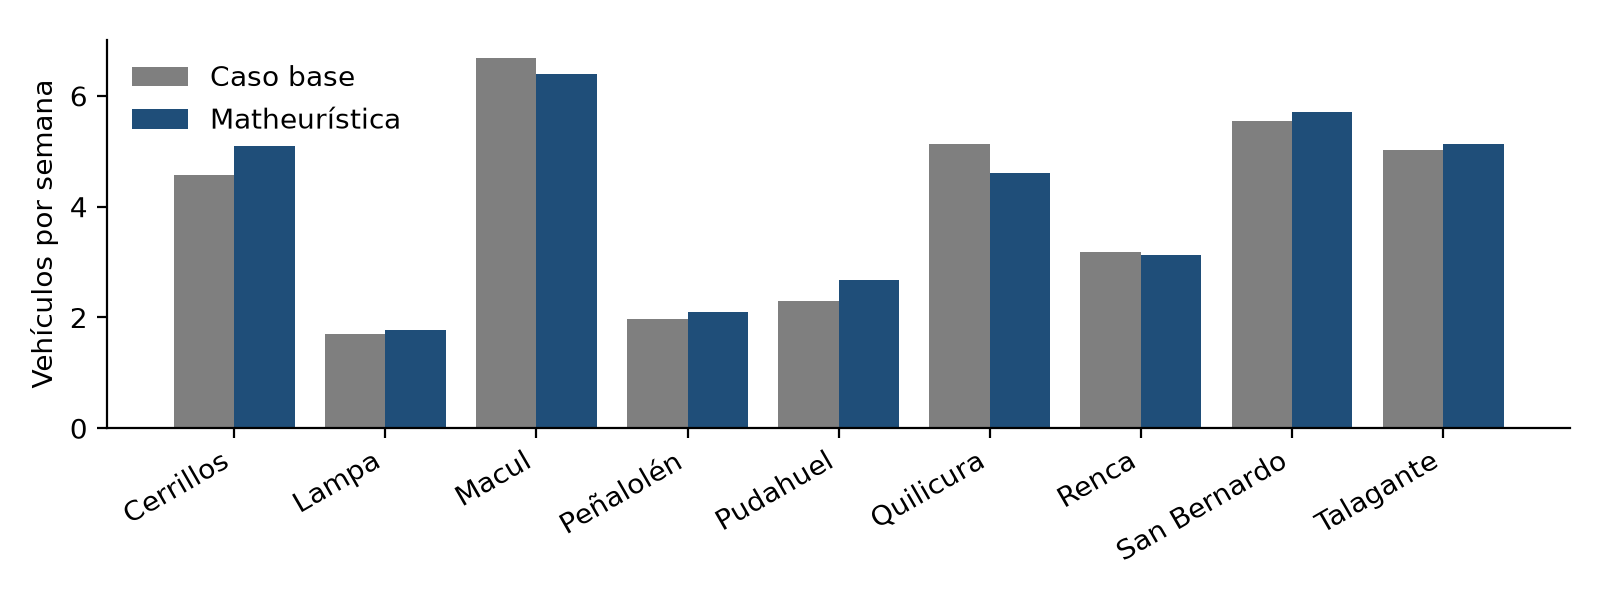
\includegraphics[width=0.9\textwidth]{figures/fig_bases.png}
\caption{Vehículos asignados a cada base, promedio de las 40 semanas.}\label{fig:bases}
\end{figure}

\parrafo{Solicitudes difíciles (objetivo O2).} De las 287 solicitudes que la matheurística externaliza en las 40 semanas, 253 también las externaliza el caso base, lo que indica que la dificultad es de la solicitud y no del método. Tienen un perfil claro: el 64\,\% son insumos y el 35\,\% equipos de retorno; su cantidad media es de 68,5 unidades, contra 32,1 del total; el 99\,\% tiene una ventana de retiro de una hora o menos, y el 40\,\% abre su retiro antes de las 09:00. Son solicitudes que necesitan un furgón o dos vehículos a la vez en un intervalo corto, justo cuando la flota de furgones está ocupada. Las de insumo son además las más baratas de externalizar (\$190.000), por lo que el modelo las elige primero cuando la capacidad no alcanza.

\parrafo{Aporte de la generación de columnas.} En la primera vuelta, el VND sobre la solución del caso base ahorra en promedio un 5,9\,\%; las vueltas siguientes, con generación de columnas, maestro y post-optimización, llevan el ahorro al 9,9\,\%. En cada semana se hacen entre 10 y 16 rondas de pricing, que agregan en promedio 2.450 rutas de costo reducido negativo a un pool final de unas 18.100. Esas rutas bajan la cota de la relajación lineal un 14\,\% respecto de la obtenida solo con las rutas del GRASP. La brecha entre la solución final y esa cota es de 10,7\,\% en promedio (8,1 a 12,8\,\%), contra 15,1\,\% en la versión anterior. Como el pricing es heurístico, la cota vale para el pool generado y no para el problema completo: indica que el maestro aprovecha bien las rutas disponibles, no que la solución esté a menos de 10,7\,\% del óptimo.

\parrafo{Validación.} Además de verificar la factibilidad, el validador revisa la coherencia económica de cada solución. En 35 de las 40 semanas no hay ninguna alerta. En las otras cinco hay seis: insumos de más de 70 unidades externalizados aunque había vehículos pagados sin salir ese día. Atenderlos exige dividirlos entre dos o tres de esos vehículos en la misma ventana de una hora, combinación que la post-optimización, que inserta un tramo a la vez, no prueba. Es una mejora pendiente acotada: valdría a lo más \$1,1 millones en total en las 40 semanas.
